\documentclass[10pt]{beamer}
\usepackage{amsmath}
\usepackage{amsthm}
\usepackage{tikz}
\usepackage{booktabs}
\usetikzlibrary{shapes.geometric, arrows}
\usepackage{listings}


\usepackage{minted}


\newcommand{\R}{\mathbb{R}}
\newcommand{\C}{\mathcal{C}}
\renewcommand{\u}{\mathbf{u}}
\renewcommand{\v}{\mathbf{v}}
\newcommand{\w}{\mathbf{w}}
\newcommand{\x}{\mathbf{x}}
\newcommand{\y}{\mathbf{y}}
\renewcommand{\b}{\mathbf{b}}
\newcommand{\e}{\mathbf{e}}
\newcommand{\s}{\mathbf{s}}


\newcommand{\A}{\mathbf{A}}
\newcommand{\B}{\mathbf{B}}
\newcommand{\W}{\mathbf{W}}

%\newtheorem{theorem}{Theorem}[section]
%\newtheorem{proposition}[theorem]{Proposition}
%\newtheorem{lemma}[theorem]{Lemma}
%\newtheorem{corollary}[theorem]{Corollary}
%
%
%\theoremstyle{definition}
%\newtheorem{definition}[theorem]{Definition}
%\newtheorem{example}[theorem]{Example}


\begin{document}
\title{Recurrent Neural Networks}
\author{Jean-Martin Albert}
\date{\today}
\maketitle

\begin{frame}{Training RNN's}
\end{frame}


\begin{frame}{The Basic RNN Cell}
\end{frame}

\defverbatim[colored]\lstI{
\begin{lstlisting}[language=Python,basicstyle=\ttfamily,keywordstyle=\color{red}]
def basic_rnn_cell(input_tensor, state_tensor, output_dimension):
  input_dimension = input_tensor.get_shape()[1]
  state_dimension = input_tensor.get_shape()[1]
  A_u = tf.Variable(shape=[input_dimension, output_dimension])
  B_u = tf.Variable(shape=[state_dimension, output_dimension])
  A_v = tf.Variable(shape=[input_dimension, state_dimension])
  B_v = tf.Variable(shape=[state_dimension, state_dimension])
  output_tensor = tf.relu(tf.matmul(input_tensor, A_u) + \
                            tf.matmul(state_tensor, B_u))
  new_state_tensor = tf.tanh(tf.matmul(input_tensor, A_v) + \
                                  tf.matmul(state_tensor, B_v))
  return output_tensor, new_state_tensor
\end{lstlisting}
}
\begin{frame}{The Basic RNN Cell (code)}
\lstI
\end{frame}


\begin{frame}{The LSTM Cell}
\end{frame}

\defverbatim[colored]\lstI{
\begin{lstlisting}[language=Python,basicstyle=\ttfamily,keywordstyle=\color{red}]
def lstm_gate(input_tensor, previous_output, port_op):
  A = tf.Variable(shape=[N, L])
  B = tf.Variable(shape=[L, L])
  b = tf.Variable(shape=[L, L])
  x = tf.matmul(input_tensor, A)+ tf.matmul(previous_output, B) + b
  return post_op(x)

def lstm_cell(input_tensor, output, state):
  F = lstm_gate(input_tensor, output, tf.sigmoid)
  I = lstm_gate(input_tensor, output, tf.sigmoid)
  O = lstm_gate(input_tensor, output, tf.sigmoid)
  S = lstm_gate(input_tensorm output, tf.tanh)
  new_state = tf.mul(output, F) + tf.mul(I, S)
  output = tf.mul(O, tf.tanh(new_state))
  return output, new_state
\end{lstlisting}
}
\begin{frame}{The LSTM Cell (code)}
\lstI
\end{frame}



\begin{frame}{The Basic GRU Cell}
\end{frame}


\defverbatim[colored]\lstI{
\begin{lstlisting}[language=Python,basicstyle=\ttfamily,keywordstyle=\color{red}]
def gru_gate(input_tensor, previous_output, port_op):
  A = tf.Variable(shape=[N, L])
  B = tf.Variable(shape=[L, L])
  b = tf.Variable(shape=[L, L])
  x = tf.matmul(input_tensor, A)+ tf.matmul(previous_output, B) + b
  return post_op(x)

def gru_cell(input_tensor, output, state):
  U = gru_gate(input_tensor, output, tf.sigmoid)
  R = gru_gate(input_tensor, output, tf.sigmoid)
  O = gru_gate(input, tf.mul(R, output))
  return tf.mul(R, output) + tf.mul((1-R)O)
\end{lstlisting}
}
\begin{frame}{The GRU Cell (code)}
\lstI
\end{frame}






\begin{frame}{A many-to-one example}
\end{frame}

\begin{frame}{A many-to-one example (model architecture)}
  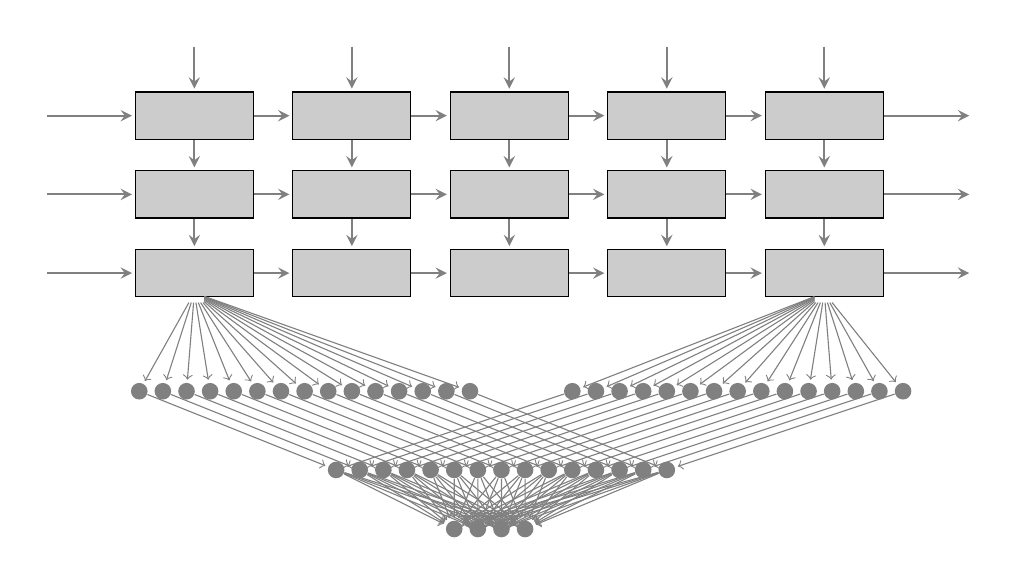
\begin{tikzpicture}[shorten >=1pt,->,draw=black!50, node distance=1cm]
      \tikzstyle{arrow} = [thick,->,>=stealth]
       \tikzstyle{every pin edge}=[<-,shorten <=1pt]
       \tikzstyle{neuron}=[circle,fill=black!50,minimum size=6pt,inner sep=0pt]

      \tikzstyle{startstop} = [rectangle, minimum width=1.5cm, minimum height=.6cm, text centered, draw=black, fill=black!20]
      \node (input) [] at (0cm,1cm) {};
      \node (output) [] at (0cm,-2.25cm) {};
      \node (s-input-A) [] at (-2cm,0cm) {};
      \node (s-output-A) [] at (10cm,0cm) {};
      \node (s-input-B) [] at (-2cm,-1cm) {};
      \node (s-output-B) [] at (10cm,-1cm) {};
      \node (s-input-C) [] at (-2cm,-2cm) {};
      \node (s-output-C) [] at (10cm,-2cm) {};
      \path[] node[startstop] (A-0) at (0cm,0cm) {};
      \path[] node[startstop] (B-0) at (0cm,-1cm) {};
      \path[] node[startstop] (C-0) at (0cm,-2cm) {};
      \draw [arrow] (input) -- (A-0);
      \draw [arrow] (s-input-A) -- (A-0);
      \draw [arrow] (s-input-B) -- (B-0);
      \draw [arrow] (s-input-C) -- (C-0);
      \draw [arrow] (A-0) -- (B-0);
      \draw [arrow] (B-0) -- (C-0);
      %\draw [arrow] (C) -- (output);

       \foreach \i/\j in {1/0,2/1,3/2,4/3}
       {
         \node (input-\i) [] at (2*\i cm,1cm) {};
         \node (output-\i) [] at (2*\i cm,-2.25cm) {};
         \path[] node[startstop] (A-\i) at (2*\i cm,0cm) {};
         \path[] node[startstop] (B-\i) at (2*\i cm,-1cm) {};
         \path[] node[startstop] (C-\i) at (2*\i cm,-2cm) {};
         \draw [arrow] (A-\i) -- (B-\i);
         \draw [arrow] (B-\i) -- (C-\i);
         \draw [arrow] (input-\i) -- (A-\i);
         \draw [arrow] (A-\j) -- (A-\i);
         \draw [arrow] (B-\j) -- (B-\i);
         \draw [arrow] (C-\j) -- (C-\i);
         %5\draw [arrow] (C-\i) -- (output-\i);
       }
       \draw [arrow] (A-4) -- (s-output-A);
       \draw [arrow] (B-4) -- (s-output-B);
       \draw [arrow] (C-4) -- (s-output-C);

       \foreach \name / \x in {1,...,15} {
           \path[xshift=-1cm]
               node[neuron] (I-\name) at (0.3*\x,-3.5cm) {};
               \path (output) edge (I-\name);
               }

       \foreach \name / \x in {1,...,15} {
           \path[xshift=4.5cm]
               node[neuron] (J-\name) at (0.3*\x,-3.5cm) {};
              \path (output-4) edge (J-\name); }

       \foreach \name / \x in {1,...,15}{
           \path[xshift=1.5cm]
               node[neuron] (K-\name) at (0.3*\x,-4.5cm) {};
          \path (I-\name) edge (K-\name);
          \path (J-\name) edge (K-\name); }

          \foreach \name / \x in {1,...,4}{
              \path[xshift=3cm] node[neuron] (O-\name) at (0.3*\x,-5.25cm) {};
              \foreach \j in {1,...,15}{
             \path (K-\j) edge (O-\name);}
             }
  \end{tikzpicture}

\end{frame}


\defverbatim[colored]\lstI{
\begin{lstlisting}[language=Python,basicstyle=\ttfamily,keywordstyle=\color{red}]
SEQ_LENGTH = 256
E_DIM = 128
STATE_DIM = 512
NUM_CLASSES = 4
def inference():
    model_input = tf.placeholder('uint8', shape=[None, SEQ_LENGTH])
    _ = tf.one_hot(Globals.model_input, depth=E_DIM, axis=-1)
    _ = tf.reshape(_, [-1, SEQ_LENGTH, E_DIM])
    fw = multi_layer_rnn(N_LAYERS, STATE_DIM)
    bw = multi_layer_rnn(N_LAYERS, STATE_DIM)
    output, _ = tf.nn.bidirectional_dynamic_rnn(fw, bw, _, dtype=tf.float32)
    fw_output = tf.reshape(output[0][:, -1:], [-1, STATE_DIM])
    bw_output = tf.reshape(output[1][:, :1], [-1, STATE_DIM])
    f = project(fw_output, E_DIM)
    b = project(bw_output, E_DIM)
    e = tf.add(f, b)
    Globals.model_output = project(e, NUM_CLASSES)
    Globals.prediction = tf.cast(tf.argmax(Globals.model_output, 1), tf.uint8)
    return Globals.model_input, Globals.model_output
\end{lstlisting}
}

\begin{frame}{A many-to-one example (code)}
\lstI
\end{frame}



\begin{frame}{A many-to-many example}
\end{frame}

\begin{frame}{A many-to-many example (model architecture)}
  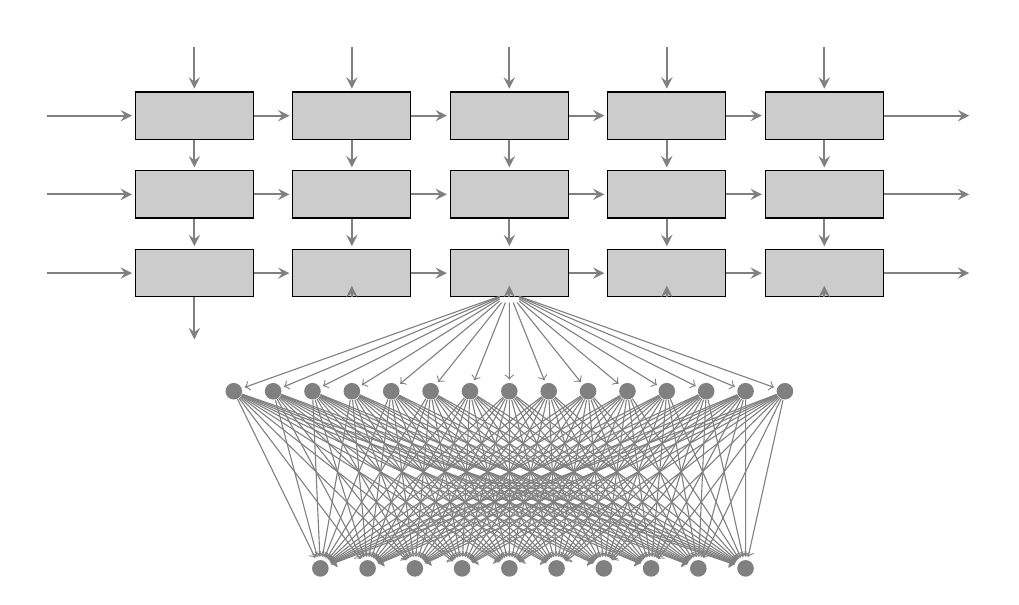
\begin{tikzpicture}[shorten >=1pt,->,draw=black!50, node distance=1cm]
      \tikzstyle{arrow} = [thick,->,>=stealth]
      \tikzstyle{startstop} = [rectangle, minimum width=1.5cm, minimum height=.6cm, text centered, draw=black, fill=black!20]
      \tikzstyle{neuron}=[circle,fill=black!50,minimum size=6pt,inner sep=0pt]

      \node (input) [] at (0cm,1cm) {};
      \node (output) [] at (0cm,-3cm) {};
      \node (s-input-A) [] at (-2cm,0cm) {};
      \node (s-output-A) [] at (10cm,0cm) {};
      \node (s-input-B) [] at (-2cm,-1cm) {};
      \node (s-output-B) [] at (10cm,-1cm) {};
      \node (s-input-C) [] at (-2cm,-2cm) {};
      \node (s-output-C) [] at (10cm,-2cm) {};
      \path[] node[startstop] (A-0) at (0cm,0cm) {};
      \path[] node[startstop] (B-0) at (0cm,-1cm) {};
      \path[] node[startstop] (C-0) at (0cm,-2cm) {};
      \draw [arrow] (input) -- (A-0);
      \draw [arrow] (s-input-A) -- (A-0);
      \draw [arrow] (s-input-B) -- (B-0);
      \draw [arrow] (s-input-C) -- (C-0);
      \draw [arrow] (A-0) -- (B-0);
      \draw [arrow] (B-0) -- (C-0);
      \draw [arrow] (C-0) -- (output);

       \foreach \i/\j in {1/0,2/1,3/2,4/3}
       {
         \node (input-\i) [] at (2*\i cm,1cm) {};
         \node (output-\i) [] at (2*\i cm,-2.25cm) {};
         \path[] node[startstop] (A-\i) at (2*\i cm,0cm) {};
         \path[] node[startstop] (B-\i) at (2*\i cm,-1cm) {};
         \path[] node[startstop] (C-\i) at (2*\i cm,-2cm) {};
         \draw [arrow] (A-\i) -- (B-\i);
         \draw [arrow] (B-\i) -- (C-\i);
         \draw [arrow] (input-\i) -- (A-\i);
         \draw [arrow] (A-\j) -- (A-\i);
         \draw [arrow] (B-\j) -- (B-\i);
         \draw [arrow] (C-\j) -- (C-\i);
         \draw [arrow] (C-\i) -- (output-\i);
       }
       \draw [arrow] (A-4) -- (s-output-A);
       \draw [arrow] (B-4) -- (s-output-B);
       \draw [arrow] (C-4) -- (s-output-C);

       \foreach \name / \x in {1,...,15}{
           \path[xshift=0cm]
               node[neuron] (K-\name) at (0.5*\x,-3.5cm) {};
          \path (output-2) edge (K-\name);
          %\path (J-\name) edge (K-\name);
          }

          \foreach \name / \x in {1,...,10}{
              \path[xshift=1cm] node[neuron] (O-\name) at (0.6*\x,-5.75cm) {};
              \foreach \j in {1,...,15}{
             \path (K-\j) edge (O-\name);}
             %\path (J-\name) edge (K-\name);
             }
  \end{tikzpicture}
\end{frame}


\defverbatim[colored]\lstI{
\begin{lstlisting}[language=Python,basicstyle=\ttfamily,keywordstyle=\color{red}]
SEQ_LENGTH = 256
E_DIM = 128
STATE_DIM = 512
N_LAYERS = 3

def inference():
    model_input = tf.placeholder('uint8', shape=[None, SEQ_LENGTH])
    _ = tf.one_hot(Globals.model_input, depth=E_DIM, axis=-1)
    encode = multi_layer_rnn(N_LAYERS, STATE_DIM)
    state_tuple = tuple(tf.unstack(Globals.initial_state, axis=0))
    output, state = tf.nn.dynamic_rnn(encode, _,
                                      dtype=tf.float32,
                                      initial_state=state_tuple)
    output = tf.reshape(output, [-1, STATE_DIM])
    output = project(output, E_DIM)
    out = tf.cast(tf.argmax(output, 1), tf.uint8)
    out = tf.reshape(out, [-1, SEQ_LENGTH])
    Globals.generated_sequence = out
    Globals.generated_characters = tf.nn.softmax(output)
    Globals.model_output = output
    Globals.state = state
\end{lstlisting}
}

\begin{frame}{A many-to-one example (code)}
\lstI
\end{frame}

\defverbatim[colored]\lstI{
\begin{lstlisting}[language=Python,basicstyle=\ttfamily,keywordstyle=\color{red}]
def generate_text(length, session=None):
    generated_text = ''
    character = [[ord(' ')]]
    istate = np.zeros([N_LAYERS, 1, STATE_DIM])
    while len(generated_text) < length:
        feed_dict = {Globals.model_input: character,
                     Globals.initial_state: istate}
        next_char, state = session.run([Globals.generated_characters,
                                        Globals.state],
                                       feed_dict=feed_dict)
        next_char = np.asarray(next_char).astype('float64')
        next_char = next_char / next_char.sum()
        op = np.random.multinomial
        next_char_id = op(1, next_char.squeeze(), 1).argmax()
        next_char_id = next_char_id if chr(next_char_id) in \
                          string.printable else ord(" ")
        generated_text += chr(next_char_id)
        character = [[next_char_id]]
        istate = state
    return generated_text
\end{lstlisting}
}


\begin{frame}{A many-to-many example (text generating)}
\lstI
\end{frame}

 \begin{frame}{Many-to-one-to-many example}

\begin{itemize}
\item  A recurrent neural network that can sort sequences
\item Two parts: an encoder, and a decoder
\item The encoder encodes sequences into fixed length vectors
\item The decoder transforms this vector into a sorted list of numbers.
\end{itemize}

 \end{frame}



 \begin{frame}{Many-to-one-to-many example}

   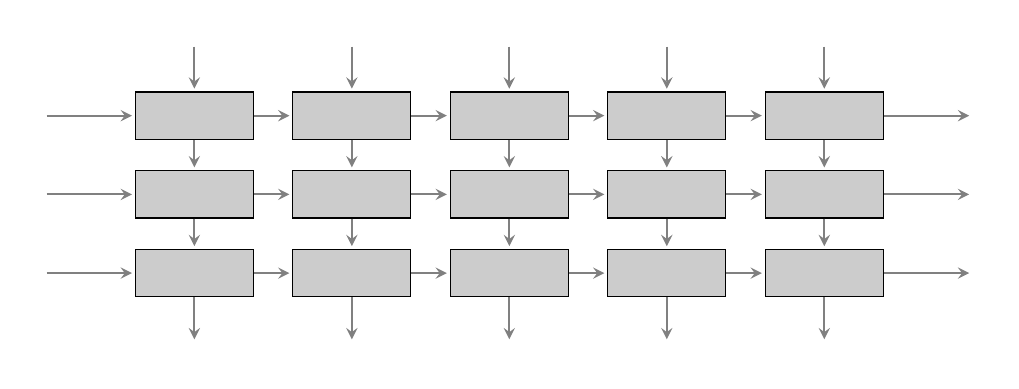
\begin{tikzpicture}[shorten >=1pt,->,draw=black!50, node distance=1cm]
       \tikzstyle{arrow} = [thick,->,>=stealth]
       \tikzstyle{startstop} = [rectangle, minimum width=1.5cm, minimum height=.6cm, text centered, draw=black, fill=black!20]
       \node (input) [] at (0cm,1cm) {};
       \node (output) [] at (0cm,-3cm) {};
       \node (s-input-A) [] at (-2cm,0cm) {};
       \node (s-output-A) [] at (10cm,0cm) {};
       \node (s-input-B) [] at (-2cm,-1cm) {};
       \node (s-output-B) [] at (10cm,-1cm) {};
       \node (s-input-C) [] at (-2cm,-2cm) {};
       \node (s-output-C) [] at (10cm,-2cm) {};
       \path[] node[startstop] (A-0) at (0cm,0cm) {};
       \path[] node[startstop] (B-0) at (0cm,-1cm) {};
       \path[] node[startstop] (C-0) at (0cm,-2cm) {};
       \draw [arrow] (input) -- (A-0);
       \draw [arrow] (s-input-A) -- (A-0);
       \draw [arrow] (s-input-B) -- (B-0);
       \draw [arrow] (s-input-C) -- (C-0);
       \draw [arrow] (A-0) -- (B-0);
       \draw [arrow] (B-0) -- (C-0);
       \draw [arrow] (C-0) -- (output);

        \foreach \i/\j in {1/0,2/1,3/2,4/3}
        {
          \node (input-\i) [] at (2*\i cm,1cm) {};
          \node (output-\i) [] at (2*\i cm,-3cm) {};
          \path[] node[startstop] (A-\i) at (2*\i cm,0cm) {};
          \path[] node[startstop] (B-\i) at (2*\i cm,-1cm) {};
          \path[] node[startstop] (C-\i) at (2*\i cm,-2cm) {};
          \draw [arrow] (A-\i) -- (B-\i);
          \draw [arrow] (B-\i) -- (C-\i);
          \draw [arrow] (input-\i) -- (A-\i);
          \draw [arrow] (A-\j) -- (A-\i);
          \draw [arrow] (B-\j) -- (B-\i);
          \draw [arrow] (C-\j) -- (C-\i);
          \draw [arrow] (C-\i) -- (output-\i);
        }
        \draw [arrow] (A-4) -- (s-output-A);
        \draw [arrow] (B-4) -- (s-output-B);
        \draw [arrow] (C-4) -- (s-output-C);

   \end{tikzpicture}
 \end{frame}


 \defverbatim[colored]\lstI{
 \begin{lstlisting}[language=Python,basicstyle=\ttfamily,keywordstyle=\color{red}]
   SEQ_LENGTH = 256
   E_DIM = 128
   STATE_DIM = 512
   N_LAYERS = 4

   def inference():
       model_input = tf.placeholder('uint8',
                                    shape=[None, SEQ_LENGTH])
       _ = tf.one_hot(model_input, depth=E_DIM, axis=-1)
       _ = tf.reshape(_, [-1, SEQ_LENGTH, E_DIM])
       encode = multi_layer_rnn(N_LAYERS, STATE_DIM)
       OP = tf.nn.dynamic_rnn
       encoded_input, state = OP(encode,_,dtype=tf.float32)
       Globals.encoder_output = state
       with tf.variable_scope('decoder'):
           training_decoder_input = tf.zeros_like(Globals.model_input)
           _ = tf.one_hot(training_decoder_input, depth=E_DIM, axis=-1)
           _ = tf.reshape(_, [-1, SEQ_LENGTH, E_DIM])
           decode = multi_layer_rnn(N_LAYERS, STATE_DIM)
           decoded_output, state = tf.nn.dynamic_rnn(decode, _,
                                                     dtype=tf.float32,
                                                     initial_state=state)
           decoded_output = tf.reshape(decoded_output, [-1, STATE_DIM])
           output = project(decoded_output, E_DIM)
           out = tf.cast(tf.argmax(output, 1), tf.uint8)
           out = tf.reshape(out, [-1, SEQ_LENGTH])
           Globals.training_decoder_input = training_decoder_input
           Globals.model_output = output
           Globals.prediction = out
           Globals.decoder = decode
           Globals.decoder_input = _
 \end{lstlisting}
 }
 \begin{frame}{Many-to-one-to-many example code}
   \lstI
 \end{frame}



\end{document}
